\chapter{HIGH LEVEL DESIGN}
\label{chp:high_level_design}
This chapter is about creating an implementation using the subcomponents mentioned in the previous chapter. The rest of the chapter is organized as follows. In Section~\ref{sec:system_design}, We will look at the system design (everything higher than a single processing element). In Section~\ref{sec:pe_design}, we will look at our processing element design. In Section~\ref{sec:file_format}, we will look at the file format. In Section~\ref{sec:latency}, we will look at how to deal with memory latency. Finally, in Section~\ref{sec:results}, we look at the results achieve from the implementation.
\section{System Design}
\label{sec:system_design}
Because each processing element acts independently during the SpMV computation it is fairly easy to come up with a high level organization. Systolic arrays work well on FPGAs \cite{prelim:johnson}. So we will use a simple 1-D systolic array for communication (See figure~\ref{fig:systolic_array}). The high amount of computation to instructions means the $O(p)$ time to send instructions is negligible. In addition, each PE connects to the shared memory and external memory. This platform has 16 virtual ports (8, 300Mhz ports multiplexed into 16 150Mhz virtual ports).
\begin{figure}
    \centering
    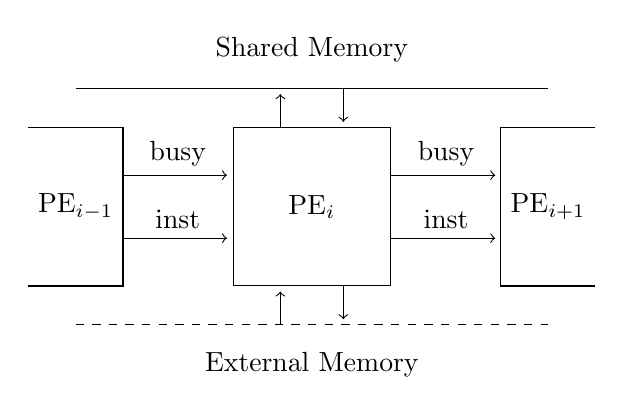
\begin{tikzpicture}
        \node (pe) at (0,0) [draw,minimum width=2cm,minimum height=2cm]{PE$_{i}$};
        \node(left) at (-3,0) [minimum width=1cm,minimum height=2cm]{PE$_{i-1}$};
        \draw (left.north west) -- (left.north east) -- (left.south east) -- (left.south west);
        \node(right) at (3,0) [minimum width=1cm,minimum height=2cm]{PE$_{i+1}$};
        \draw (right.north east) -- (right.north west) -- (right.south west) -- (right.south east);
        \node at (0, 2) {Shared Memory};
        \node at (0, -2) {External Memory};
        \draw (-3,1.5) -- (3,1.5);
        \draw [dashed] (-3,-1.5) -- (3,-1.5);

        \draw [->,shorten >=2pt](left.east |- 0,.4) -- (pe.west |- 0,.4) node [midway,above]{busy};
        \draw [->,shorten >=2pt](left.east |- 0,-.4) -- (pe.west |- 0,-.4) node [midway,above]{inst};

        \draw [->,shorten >=2pt](pe.east |- 0,.4) -- (right.west |- 0,.4) node [midway,above]{busy};
        \draw [->,shorten >=2pt](pe.east |- 0,-.4) -- (right.west |- 0,-.4) node [midway,above]{inst};

        \draw [->,shorten >=2pt](pe.north -| -.4,0) -- (0,1.5 -| -.4,0);
        \draw [->,shorten >=2pt](0,1.5 -| .4,0) -- (pe.north -| .4,0);

        \draw [->,shorten >=2pt](0,-1.5 -| -.4,0) -- (pe.south -| -.4,0);
        \draw [->,shorten >=2pt](pe.south -| .4,0) -- (0,-1.5 -| .4,0);

    \end{tikzpicture}
    \caption[The 1-D Systolic array structure of processing elements.]{The processing element are arranged in a simple 1-D systolic array.}
    \label{fig:systolic_array}
\end{figure}
\section{Processor Design}
\label{sec:pe_design}
\begin{table}
    \centering
    \caption{The opcodes for the SpMV processor.}
    \label{tbl:opcodes}
    \begin{tabular}{|m{1cm}|c|m{2cm}|c|m{5cm}|}
        \hline
        opcode & name & arg1 & arg2 & description \\
        \hline
        0000 & NOP & N/A & N/A & This is the default signal sent to the PEs. \\
        \hline
        0001 & RESET & N/A & N/A & This reset eliminates the need for a seperate reset signal to be routed to all the PEs.\\
        \hline
        0010 & WRITE & register address & data & This loads data into the specified register.\\
        \hline
        0011 & LOAD\_DELTA\_CODES & N/A & N/A & This loads the delta codes into the cooresponding lookup table in the decoder.\\
        \hline
        0100 & LOAD\_PREFIX\_CODES & N/A & N/A & This loads the prefix codes into the cooresponding lookup table in the decoder.\\
        \hline
        0101 & LOAD\_COMMON\_VALUES & N/A & N/A & This loads the 8,192 most common values into the shared memory.\\
        \hline
        0110 & EXECUTE\_SPMV & N/A & N/A & This instructs the PE(s) to perform the SpMV operation.\\
        \hline
        0111 & READ & register address & N/A & This instructs the PE to return the data on the specified register.\\
        \hline
        1000 & RETURN & register address & data & This is sent from the PE after the READ instruction is received.\\
        \hline
        1001-1111 & RESERVED & N/A & N/A & N/A \\
        \hline
%

    \end{tabular}
\end{table}
One way to describe our processing element is that it is a very small instruction set processor for SpMV. However, the instructions are mostly for organization of the hardware not execution like in other work [\cite{prelim:good}]. The instructions are 64 bits wide and consist of 4 parts: a 4-bit opcode, a 5-bit PE ID, a 4-bit first argument, and a 51-bit second argument. The opcodes described in Table~\ref{tbl:opcodes}.

\begin{table}
    \centering
    \caption{The registers in each SpMV processing element.}
    \label{tbl:registers}
    \begin{tabular}{|c|c|m{8cm}|}
        \hline
        Register & Name & Description\\
        \hline
        0 & $y$ vector address & The address to store the next $y$ value. \\
        \hline
        1 & ending $y$ vector address & The one over last address of the last $y$ value.\\
        \hline
        2 & $x$ vector address & The static address of the $x$ vector.\\
        \hline
        3 & nnz MAC count down & Starts at nnz - 1 and decreases by one for each value that enter the MAC.\\
        \hline
        4 & index opcodes address & The address of the next 8 byte chunk to request from the index opcodes stream. In the LOAD\_DELTA\_CODES, LOAD\_PREFIX\_CODES, and LOAD\_COMMON\_CODES operations this register stores the address of the next 8-byte chuck to read in.\\
        \hline
        5 & index argument address & The address of the next 8 byte chunk to request from the index argument stream. In the LOAD\_DELTA\_CODES, LOAD\_PREFIX\_CODES, and LOAD\_COMMON\_CODES operations this register stores the address of where the next element is stored in on-chip memory.\\
        \hline
        6 & fzip opcodes address & The address of the next 8 byte chunk to request from the fzip opcodes stream.\\
        \hline
        7 & fzip argument address & The address of the next 8 byte chunk to request from the fzip argument streams.\\
        \hline
        8 & ending index opcodes address & The one over last address of the space allocated to the index opcodes stream. In the LOAD\_DELTA\_CODES, LOAD\_PREFIX\_CODES, and LOAD\_COMMON\_CODES operations this register stores the one over last address of the data being read in.\\
        \hline
        9 & ending index argument address & The one over last address of the space allocated to the index arguments stream. In the LOAD\_DELTA\_CODES, LOAD\_PREFIX\_CODES, and LOAD\_COMMON\_CODES operations this register stores the one over last address of the on-chip memory.\\
        \hline
        10 & ending fzip opcodes address & The one over last address of the space allocated to the fzip opcodes stream.\\
        \hline
        11 & ending fzip arguments address & The one over last address of the space allocated to the fzip arguments stream.\\
        \hline
        12 & nnz index count down & Starts at nnz - 1 and decreases by one for each index pair that exits the decoder.\\
        \hline
        13 & nnz fzip count down & Starts at nnz - 1 and decreases by one for each floating point value that exits the decoder.\\
        \hline
        14-15 & reserved & Used for debugging.\\
        \hline
    \end{tabular}

\end{table}

There are 14, 48-bit registers on each processing element. The function of each register is described in Table~\ref{tbl:registers}. All of these registers serve a purpose during the main stage (SPMV\_EXECUTE). Registers 4, 5, 8 and 9 also have a function in the other stages (LOAD\_DELTA\_CODES, LOAD\_PREFIX\_CODES, LOAD\_PREFIX\_CODES, and LOAD\_COMMON\_VALUES).

The debug registers give a better understanding of the operation of the processing element during the SpMV operation.

\section{File format}
\label{sec:file_format}
We looked at previous file formats like gzip [\cite{prelim:deutsch}] to help create a new file format. We start with a 256-byte header. This header has reserved values for future versions, pointers to the sections of the file, and other values about the matrix or compression streams. Each value in the header is 8-bytes. The specification of each value is described in Table~\ref{tbl:header}.

\begin{table}
    \centering
    \caption{The header for our sparse matrix compression file format (SMC).}
    \label{tbl:header}
    \begin{tabular}{|ccm{6cm}|}
        \hline
        Number & Field & Description\\
        \hline
        0 & RESERVED & \\
        \hline
        1 & width & The width of the matrix.\\
        \hline
        2 & height & The height of the matrix.\\
        \hline
        3 & nnz & Number of non-zero values in the matrix.\\
        \hline
        4 & spmCodeSTreamBitLength & Number of bits in the sparse pattern code stream.\\
        \hline
        5 & spmArgumentStreamBitLength & Number of bit in the sparse pattern argument stream.\\
        \hline
        6 & fzipCodeStreamBitLength & Number of bits in the fzip (floating point) code stream.\\
        \hline
        7 & fzipArgumentStreamBitLength & Number of bits in the fzip (floating point) argument stream.\\
        \hline
        8-15 & RESERVED & \\
        \hline
        16 & spmCodesPtr & Offset from the start of the file to the start of the delta codes (will always be 256).\\
        \hline
        17 & fzipCodesPtr & offset from the start of the file to the start of the fzip codes (will always be 4352).\\
        \hline
        18 & commonDoublesPtr & Offset from the start of the file to the start of the 8,192 common floating point values (will always be 12544).\\
        \hline
        19 & spmCodeStreamPtr & Offset from the start of the file to the start of the sparse pattern matrix code stream.\\
        \hline
        20 & spmArgumentStreamPtr & Offset from the start of the file to the start of the sparse pattern matrix argument stream.\\
        \hline
        21 & fzipCodeStreamPtr & Offset from the start of the file to the start of the fzip code stream.\\
        \hline
        22 & fzipArgumentStream Ptr & Offset from the start of the file to the start of the fzip argument stream.\\
        \hline
        23 & size & The total number of bytes in the file. \\
        \hline
        24-31 & RESERVED & \\
        \hline
    \end{tabular}
\end{table}

Three constant length sections after the header. First, the codes for the sparse pattern matrix compression. Second, the codes for the fzip compression. Third, the common floating point values (also for fzip compression). These sections will take a small fraction of the total file space for large matrices. For this reason we choose not to try to compress these sections further and just leave them as simple as possible.

Four data streams follow after all the decoding information, the code and argument stream for the indices and the code and argument streams for the floating point values. These streams have a variable bit length but there exists extra buffer bits to get to a 8 byte boundary. To make the design of the decoders easier there is at least 8 bytes of buffer space. For the fzip argument stream, there is at least 48 bytes of buffer space to increase throughput of decoding floating point values.

\section{Memory Latency}
\label{sec:latency}
\begin{figure}
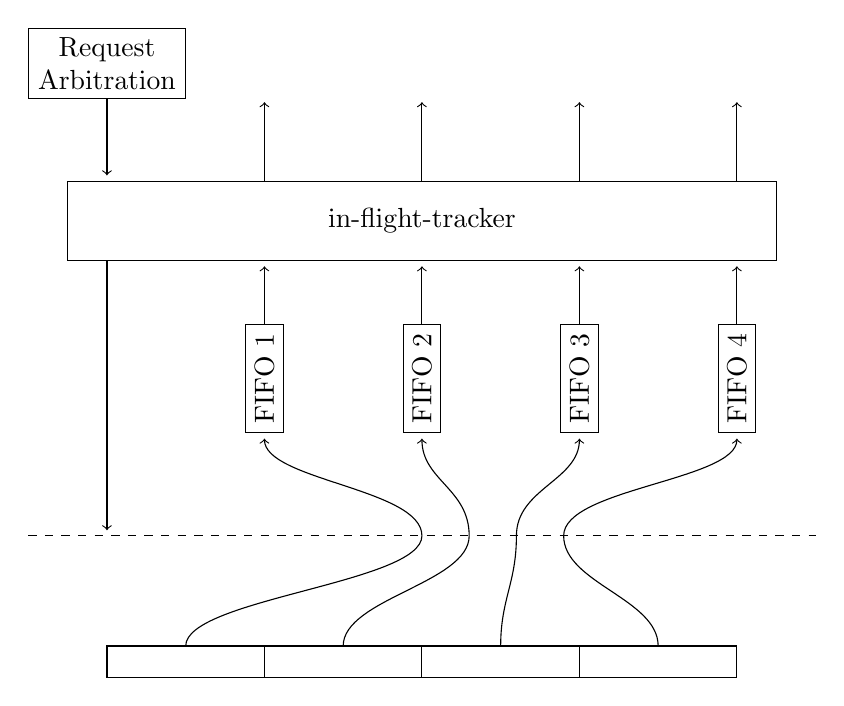
\begin{tikzpicture}[xscale=2,yscale=2]
\node(req) at (0,0) [draw]{\shortstack{Request\\Arbitration}};
\node(tracker) at (2,-1) [draw, minimum width=9cm, minimum height=1cm]{in-flight-tracker};
\node(f1) at (1, -2) [draw,rotate=90]{FIFO 1};
\node(f2) at (2, -2) [draw,rotate=90]{FIFO 2};
\node(f3) at (3, -2) [draw,rotate=90]{FIFO 3};
\node(f4) at (4, -2) [draw,rotate=90]{FIFO 4};
\draw[dashed] (-.5,-3) -- (4.5,-3);
\draw (0,-3.7) -- (4,-3.7) -- (4,-3.9) -- (0,-3.9) -- cycle;
\draw (1,-3.7) -- (1,-3.9);
\draw (2,-3.7) -- (2,-3.9);
\draw (3,-3.7) -- (3,-3.9);

\draw [->,shorten >=2pt] (req) -- (tracker.north -| req);
\draw [->,shorten >=2pt] (tracker.south -| req) -- (0,-3 -| req);
\draw [<-,shorten <=2pt] (f1.west) .. controls +(0,-.3) and +(0,.3) .. (2,-3) .. controls +(0,-.3) and +(0,.3) .. (.5,-3.7);
\draw [<-,shorten <=2pt] (f2.west) .. controls +(0,-.3) and +(0,.3) .. (2.3,-3) .. controls +(0,-.3) and +(0,.3) .. (1.5,-3.7);
\draw [<-,shorten <=2pt] (f3.west) .. controls +(0,-.3) and +(0,.3) .. (2.6,-3) .. controls +(0,-.3) and +(0,.3) .. (2.5,-3.7);
\draw [<-,shorten <=2pt] (f4.west) .. controls +(0,-.3) and +(0,.3) .. (2.9,-3) .. controls +(0,-.3) and +(0,.3) .. (3.5,-3.7);

\draw [->,shorten >=2pt] (f1) -- (tracker.south -| f1);
\draw [->,shorten >=2pt] (f2) -- (tracker.south -| f2);
\draw [->,shorten >=2pt] (f3) -- (tracker.south -| f3);
\draw [->,shorten >=2pt] (f4) -- (tracker.south -| f4);

\draw [->] (tracker.north -| f1) -- +(0,.5);
\draw [->] (tracker.north -| f2) -- +(0,.5);
\draw [->] (tracker.north -| f3) -- +(0,.5);
\draw [->] (tracker.north -| f4) -- +(0,.5);

\end{tikzpicture}
\caption{Memory request arbitration.}
\label{fig:memory_latency}
\end{figure}
Dealing with memory latency is not trivial. The difficulty lies in the fact we are reading 4 streams at different rates. Our platform has a 700 clock cycle external memory latency. We created a general approach with one tweak to achieve high throughput under these conditions.

The hardware consists of 3 parts. First, 4 FIFOs buffer the memory responses of the 4 different streams. Second, an `in-flight-tracker' keeps track of the number of requests to ensure the FIFOs never overflow or have to stall the memory. Third, the request logic determines which (if any) stream should be read from on the current clock cycle.

We use a round robin for request arbitration. We use 3 different signals to determine when to move to the next stream: the tracker information, FIFO saturation and time. First, if the tracker indicates that the limit of in-flight requests has been reached the request arbiter switches to the next stream. Second, if the FIFO corresponding to the to the current stream is half full (indicating that the stream does not need to be read from so often) then the request arbiter switches to the next stream. Third, a timer insures each well get at most 32 requests before the request arbiter switches to the next stream.

\par In practice this still does not achieve good throughput when computing memory bound (difficult to compress) matrices. The problem is that the fzip argument stream (the non-encoded bits or common value index stream) ends up starving and slows down the decoder. To solve this we give priority to this stream by only moving from it when the tracker indicates no more in flight messages can be accepted. This means the timer and the FIFO saturation will not cause the request arbiter to stop reading this stream.
%TODO: explain why
\section{Results}
\label{sec:results}
$R^3$, our previous work, achieved up to 13.6 GFLOPS and an average performance of 7.6 GFLOPS. In this work we were able to achieve up to 16.6 GFLOPS and achieve an average performance of 9.4 GFLOPS.

\begin{figure*}
\centering
\begin{tikzpicture}[scale=1]

 \ifthenelse{\equal{\blackandwhite}{true}}{
	\tikzstyle{yellowStar}=[draw, diamond, fill=black!65, inner sep =1.5pt];
	\tikzstyle{blueGreenDiamond}=[draw, diamond, fill=black!75, inner sep =1.5pt];
	\tikzstyle{greenSquare}=[draw, rectangle, fill=black!50, inner sep =2.5pt];
	\tikzstyle{blueTriangle}=[draw, regular polygon, regular polygon sides=3, fill=black!35, inner sep =1.5pt];
 }{
	\tikzstyle{yellowStar}=[draw, star, star points=5, fill=yellow, inner sep =1.5pt];
	%\tikzstyle{blueGreenDiamond}=[draw, diamond, fill=green!60!blue, inner sep =1.5pt];
	\tikzstyle{blueGreenDiamond}=[draw, diamond, fill=black, inner sep =1.5pt];
	\tikzstyle{greenSquare}=[draw, rectangle, fill=green, inner sep =2.5pt];
	\tikzstyle{blueTriangle}=[draw, regular polygon, regular polygon sides=3, fill=blue, inner sep =1.5pt];
 }

%\draw [ystep=2.0,gray,very thin, xstep = 14] (0,0) grid (12.9, 6.9);
\draw [->,thick] (0,0) to (14.5, 0);
\draw [->, thick] (0,0) to (0,7);
\foreach \x/\mat/\size in { %
0/dw8192/42K, 1/t2d\_q9/87K, 2/epb1/95K, 3/raefsky1/290K, 4/psmigr\_2/540K, 6/torso2/1M%
}
	\draw (\x cm, 1pt) -- (\x cm, -1pt) node[anchor=east,rotate=90,gray] {\shortstack{\mat (\size)}};
\foreach \x/\mat/\size in { %
5/scircuit/960K, 7/mac\_econ/1.3M, 8/qcd5\_4/1.9M, 9/mc2depi/2.1M, 10/rma10/2.3M, 11/shipsec1/3.6M, 12/dense/4M, 13/cant/4M, 14/consph/6M%
}
	\draw (\x cm, 1pt) -- (\x cm, -1pt) node[anchor=east,rotate=90] {\shortstack{\mat (\size)}};
\foreach \y/\ytext in {0/0,1/5,2/10, 3/15, 4/20, 5/25, 6/30}
	\draw (1pt, \y cm) -- (-1pt, \y cm) node[anchor=east] {$\ytext$};
%\node at (6, -.8) {Size of Matrix (Millions)};
\node at (-1, 3) [rotate=90]{Performance (Gflops)};

%R3 line
\foreach \i/\j/\k/\l in {%
0/0.42000000000000004/1/0.76,  1/0.76/2/0.6599999999999999,  2/0.6599999999999999/3/1.04,  3/1.04/4/0.9800000000000001,  4/0.9800000000000001/5/1.24,  5/1.24/6/1.28,  6/1.28/7/1.1800000000000002,  7/1.1800000000000002/8/2.56,  8/2.56/9/1.24,  9/1.24/10/2.7199999999999998,  10/2.7199999999999998/11/1.58,  11/1.58/12/2.7199999999999998,  12/2.7199999999999998/13/2.54,  13/2.54/14/1.7399999999999998
}{
 \ifthenelse{\equal{\blackandwhite}{true}}{
	\draw [black] (\i,\j) -- (\k,\l);
 }{
	\draw [red] (\i,\j) -- (\k,\l);
 }
}

%hc1 line
\foreach \i/\j/\k/\l in {%
0/0.33999999999999997/1/0.5,  1/0.5/2/0.52,  2/0.52/3/0.78,  3/0.78/4/0.78,  4/0.78/6/0.24
}{
 \ifthenelse{\equal{\blackandwhite}{true}}{
	\draw [black!65] (\i,\j) -- (\k,\l);
 }{
	\draw [brown] (\i,\j) -- (\k,\l);
 }
}

%%tesla line
%\foreach \i/\j/\k/\l in {%
%0/0.1/1/0.18,  1/0.18/2/0.16,  2/0.16/3/0.5599999999999999,  3/0.5599/5/0.6}
%	\draw <3,5>[green!60!blue] (\i,\j) -- (\k,\l);
%newline

%m2090 line
\foreach \i/\j/\k/\l in {%
5/1.2/7/1.2,  7/1.2/8/4.0,  8/4.0/9/4.4,  9/4.4/10/2.2,  10/2.2/11/2.2,  11/2.2/12/4.6,  12/4.6/13/3.4,  13/3.4/14/3.0
}{
 \ifthenelse{\equal{\blackandwhite}{true}}{
	\draw [black!50] (\i,\j) -- (\k,\l);
 }{
	\draw [green] (\i,\j) -- (\k,\l);
 }
}

%intel line
\foreach \i/\j/\k/\l in {%
5/2.4/7/4.6,  7/4.6/8/6.0,  8/6.0/9/4.2,  9/4.2/10/4.8,  10/4.8/11/2.0,  11/2.0/12/2.8,  12/2.8/13/2.4,  13/2.4/14/2.2
}{
 \ifthenelse{\equal{\blackandwhite}{true}}{
	\draw [black!35] (\i,\j) -- (\k,\l);
 }{
	\draw [blue] (\i,\j) -- (\k,\l);
 }
}

\foreach \i/\j/\k/\l in {%
    0/0.42000000000000004/1/0.78,  1/0.78/2/0.6799999999999999,  2/0.6799999999999999/3/1.1,  3/1.1/4/1.1400000000000001,  4/1.1400000000000001/5/1.3,  5/1.3/6/1.54,  6/1.54/7/1.7,  7/1.7/8/3.04,  8/3.04/9/1.8,  9/1.8/10/3.1,  10/3.1/11/3.3200000000000003,  11/3.3200000000000003/12/3.08,  12/3.08/13/3.1399999999999997,  13/3.1399999999999997/14/2.2
}{
 \ifthenelse{\equal{\blackandwhite}{true}}{
	\draw [black!35] (\i,\j) -- (\k,\l);
 }{
	\draw [black] (\i,\j) -- (\k,\l);
 }
}

%\draw [dashed] (.5, -.5) -- (.5, 7) node [fill=white,inner sep=0pt, midway,below, sloped]{\small $(64K)$};

%\draw [dashed] (10.5, -.5) -- (10.5, 7)  node [fill=white,inner sep=0pt, near end,below, sloped]{\small 20MB $(2.5M)$};



%hc1 points
\foreach \i/\x/\y/\f/\q/\u in {%
0/0.083492/0.33999999999999997/1.7/0/-.2,%
1/0.17405/0.5/2.5/0/-.1,%
2/0.190106/0.52/2.6/0/-.2,%
3/0.588552/0.78/3.9/0/-.2,%
4/1.080044/0.78/3.9/0/-.2,%
6/2.066946/0.24/1.2/0/0
}{
 \ifthenelse{\equal{\blackandwhite}{true}}{
	\draw (\i,\y) node[yellowStar]{} node[fill=white,inner sep=0pt, anchor=west,rotate=30,xshift=\q cm + 3pt, yshift=\u cm] {\color{black!65} \scriptsize $\f$};
 }{
	\draw (\i,\y) node[yellowStar]{} node[fill=white,inner sep=0pt, anchor=west,rotate=30,xshift=\q cm + 3pt, yshift=\u cm] {\color{brown} \scriptsize $\f$};
 }
}	

%intel points
\foreach \i/\x/\y/\f/\q/\u in {%
5/1.917872/2.4/12/0/0,%
7/2.546778/4.6/23/0/0,%
8/3.833856/6.0/30/0/0,%
9/4.20045/4.2/21/0/-.2,%
10/4.658184/4.8/24/0/0,%
11/7.136352/2.0/10/0/0,%
12/8.0/2.8/14/0/.2,%
13/8.014766/2.4/12/0/-.2,%
14/12.02096/2.2/11/0/0
}{
 \ifthenelse{\equal{\blackandwhite}{true}}{
	\draw (\i cm,\y cm) node[blueTriangle]{} node[fill=white,inner sep=0pt, anchor=west,rotate=30,xshift=\q cm + 3pt, yshift=\u cm]{\color{black!50} \scriptsize $\f$};
 }{
	\draw (\i cm,\y cm) node[blueTriangle]{} node[fill=white,inner sep=0pt, anchor=west,rotate=30,xshift=\q cm + 3pt, yshift=\u cm]{\color{blue} \scriptsize $\f$};
 }
}

%M2090 points
\foreach \i/\x/\y/\f/\q/\u in {%
5/1.917872/1.2/6/0/-.3,%
7/2.546778/1.2/6/0/.3,%
8/3.833856/4.0/20/0/0,%
9/4.20045/4.4/22/0/0,%
10/4.658184/2.2/11/0/0,%
11/7.136352/2.2/11/0/.1,%
12/8.0/4.6/23/0/0,%
13/8.014766/3.4/17/0/0,%
14/12.02096/3.0/15/0/0
}{
 \ifthenelse{\equal{\blackandwhite}{true}}{
	\draw (\i,\y) node[greenSquare]{} node[fill=white,inner sep=0pt, anchor=west,rotate=30,xshift=\q cm + 3pt, yshift=\u cm]{\color{black!35} \scriptsize $\f$};
 }{
	\draw (\i,\y) node[greenSquare]{} node[fill=white,inner sep=0pt, anchor=west,rotate=30,xshift=\q cm + 3pt, yshift=\u cm]{\color{green!100} \scriptsize $\f$};
 }
}

%R3 points
\foreach \i/\x/\y/\f/\q/\u in {%
0/0.083492/0.42000000000000004/2.1/0/0,%
1/0.17405/0.76/3.8/0/0,%
2/0.190106/0.6599999999999999/3.3/0/0,%
3/0.588552/1.04/5.2/0/0,%
4/1.080044/0.9800000000000001/4.9/0/0,%
5/1.917872/1.24/6.2/0/0,%
6/2.066946/1.28/6.4/0/0,%
7/2.546778/1.1800000000000002/5.9/0/0,%
8/3.833856/2.56/12.8/0/0,%
9/4.20045/1.24/6.2/0/0,%
10/4.658184/2.7199999999999998/13.6/0/0,%
11/7.136352/1.58/7.9/0/0,%
12/8.0/2.7199999999999998/13.6/0/0,%
13/8.014766/2.54/12.7/0/0,%
14/12.02096/1.7399999999999998/8.7/0/0
}{
 \ifthenelse{\equal{\blackandwhite}{true}}{
	\draw (\i,\y) [fill=black]circle(3pt) node(r\i)[fill=white,inner sep=0pt, anchor=west,rotate=30,xshift=\q cm + 3pt, yshift=\u cm]{\color{black} \scriptsize $\f$}; 
 }{
	\draw (\i,\y) [fill=red]circle(3pt) node(r\i)[fill=white,inner sep=0pt, anchor=west,rotate=30,xshift=\q cm + 3pt, yshift=\u cm]{\color{red} \scriptsize $\f$};
 }
}
%new points
\foreach \i/\x/\y/\f/\q/\u in {%
0/0.083492/0.42000000000000004/2.1/0/0,%
1/0.17405/0.78/3.9/0/0,%
2/0.190106/0.6799999999999999/3.4/0/0,%
3/0.588552/1.1/5.5/0/0,%
4/1.080044/1.1400000000000001/5.7/0/0,%
5/1.917872/1.3/6.5/0/0,%
6/2.066946/1.54/7.7/0/0,%
7/2.546778/1.7/8.5/0/0,%
8/3.833856/3.04/15.2/0/0,%
9/4.20045/1.8/9.0/0/0,%
10/4.658184/3.1/15.5/0/0,%
11/7.136352/3.3200000000000003/16.6/0/0,%
12/8.0/3.08/15.4/0/0,%
13/8.014766/3.1399999999999997/15.7/0/0,%
14/12.02096/2.2/11.0/0/0
}{
 \ifthenelse{\equal{\blackandwhite}{true}}{
	\draw (\i,\y) node[greenSquare]{} node[fill=white,inner sep=0pt, anchor=west,rotate=30,xshift=\q cm + 3pt, yshift=\u cm]{\color{black!35} \scriptsize $\f$};
 }{
	\draw (\i,\y) node[blueGreenDiamond]{} node[fill=white,inner sep=0pt, anchor=west,rotate=30,xshift=\q cm + 3pt, yshift=\u cm]{\color{black!100} \scriptsize $\f$};
 }
}

\draw (4,5.5) node (key)[rectangle,minimum width=4cm, minimum height=2.7cm]{};
 \ifthenelse{\equal{\blackandwhite}{true}}{
	\node at (key) [rectangle,anchor=west, xshift=-2cm, yshift=1cm]{\tikz{\draw (0,1pt) [fill=black]circle (2.5pt);} $R^3$};
 }{
	\node at (key) [rectangle,anchor=west, xshift=-2cm, yshift=1cm]{\tikz{\draw (0,1pt) [fill=red]circle (2.5pt);} $R^3$};
 }
\node at (key) [rectangle,anchor=west, xshift=-2cm, yshift=1.7cm]{\shortstack{\tikz{\draw (0,1pt) node[blueGreenDiamond]{};} This Work}};
\node at (key) [rectangle,anchor=west, xshift=-2cm, yshift=.3cm]{\shortstack{\tikz{\draw (0,1pt) node[yellowStar]{};} \cite{prelim:nagar1} }};
%\node <3,5>at (key) [rectangle,anchor=west, xshift=-2cm, yshift=0cm]{\tikz{\draw (0,1pt) node[blueGreenDiamond]{};} Nvidia Tesla S1070};
\node at (key) [rectangle,anchor=west, xshift=-2cm, yshift=-.5cm]{\shortstack{\tikz{\draw (0,1pt) node[greenSquare]{};} Nvidia Tesla \\M2090}};
\node at (key) [rectangle,anchor=west, xshift=-2cm, yshift=-1.5cm]{\shortstack{\tikz{\draw (0,1pt) node[blueTriangle]{};} Intel E5-2690 \\(2 CPUs)}};

\end{tikzpicture}
\caption[SpMV performance on our newest design.]{$nnz$ vs Performance on each platform. As seen we achieve about a 20\% increase in performance compared to $R^3$.}
\label{fig:newResults}
\end{figure*}

Some trends do appear. Like in $R^3$ the new design does not achieve good performance on the smallest matrices. This is due to the memory latency of the platform. In fact, the smallest matrix (dw8192) is so small that all of the read requests occur before the first value is multiplied.

Another trend is that the more compressible matrices achieve the best performance. The 3 pattern matrices (qcd5\_4, rma10, and dense) achieve the best performance.

In terms of area about half of the Xilinx Virtex-6 LX760 FPGA is utilized. The uses 255K out of 948K registers, 224K out of 474K LUTs, 515 out of 720 RAM blocks, 112 out of 864 DSPs (multiplier blocks).
